\textbf{Danke an ...}
\\

%TODO: Tutorennamen hier einfügen
\begin{tabular}{l l l} 

Adrian Ackermann  & Peter Klausing  & Lisa Ragosina\\
Justus Adam  & Tim Kluge & Melanie Ramsch\\
Anna Baumgärtel  & Fabian Koller & Josephine Rehak\\
Bettina  Blasberg & Kilian Költzsch & Axel Reinicke\\
Meinhardt Branig & Nadja Konrad & Franziska Ressel\\
Anna Brauer & Max Korn & Anja Reusch\\
Markus Damm & Ben Kosmann  & Rico\\
Felix Döring  & Nikolai Kostka & Christian Riedel\\
Georg Eckert & Alexandra Krien & Christian Rose\\
Björn Einert & Sandra Kukulka & Marcel Rösler\\
Martin Eisoldt & Richard Kwasnicki & Marc Satkowski\\
Lars Engeln  & Kristian Kyas & Florian Schmidt\\
Daniel Fischer & Dirk Legler & Michael Schneider\\
Tamara Flemisch & Matthias Lehne & Lara von Schuhmann\\
Sven Goly & Adrian Lieber & Franz-Wilhelm Schumann\\
Julius Gonsior & Katja Linnemann & Patrick Stiller\\
Sara Groß & Ian Alexander List & Julian Lars Striegl\\
Anita Grützner & Willi Mentzel & Sinthujan Thanabalansingam\\
Sebastian Hahn & Sebastian Mielke & Manual Thieme\\
Thomas Hauptvogel & Richard Mörbitz & Duc Anh Trinh\\
Frank Hedecke & Emma Müller & Sebastian Vogt\\
Phillip Heisig & Vincent Nadoll & Sandra Waske\\
Marius Hogräfer & Anne-Marie Oelschläger & Stefan Weckend\\
Ulrich Huber & David Ordnung & Jens Wettlaufer\\
Christoph Jurkoswki & Dominik Pataky & Andreas Wilke\\
Christian Kabelitz & Sascha Peukert & Lucas Woltmann\\
Sebastian Kiehne & Philip Plotz & Laura Zepner\\

\end{tabular}

\addchap{Vorwort}

Hallo Uniwelt!

heißt es nun für dich als frisch Immatrikulierter, Ersti, an der TU Dresden. 
Endlich kannst du nach Jahren der Knechtschaft selbst über dich und dein Leben bestimmen. 
Wie du mit dieser Freiheit und der daraus folgenden Verantwortung zurecht kommst, lernst du schnell. 
Damit dir der Übergang leichter fällt, veranstaltet dein Fachschaftsrat die Erstsemestereinführung (ESE). 
Eine Woche lang gibt es neben Spiel und Spaß sehr viel Informatives zum Studium sowie zum Unileben allgemein. 
Dieses Heft ist ein nützlicher Ratgeber und nicht vergessen: 
\textbf{NO PANIC!} (Aus historischen Gründen hier nicht das grammatikalisch korrekte \glqq don't panic\grqq. Hinweise auf diesen grammatikalischen Fauxpas werden mit Matekästenschulden geahndet.)

Du wirst auch entdecken, dass Uni mehr ist als nur studieren. 
Neben allerlei Erstsemesterparties gibt es noch mehr zu erleben. 
Gerade prägend für die Dresdner Hochschulkultur sind die 17 Studentenclubs, wie z.B. das CountDown in der Johannstadt. 
In der Neustadt laden viele Kneipen und Clubs zu langen Nächten ein. 
Einmal im Jahr entlädt sich dieses alternative Flair während der BRN (Bunte Republik Neustadt). 
Und wem das alles viel zu hektisch ist: der fläze sich gemütlich in ein Sofa vom ASCII, dem Studentencafé der Fakultät. 
Dort kann man gut bei Kaffee und Club Mate (empfehlenswert auch die lokale Kolle-Mate!) entspannen oder versuchen doch etwas für die Uni zu tun.

Engagement wird an der TU Dresden groß geschrieben. 
Es gibt viele Hochschulgruppen die um eure Mitarbeit buhlen. 
Darunter einige politische, wie auch technische, journalistische, künstlerische und und und. Mehr dazu findest du auf der Seite des StuRa.

Dieses Heft enthält übrigens auch eine Vielzahl von Links zu relevanten Unterseiten auf den Seiten des FSR, der Uni und anderen. 
Diese sind mit Zahlen wie dieser hier \link{http://bit.ly/Vt4Ua6} versehen und ganz am Ende des Heftes gelistet. Ebenfalls kannst du auch direkt unter \url{ese.ifsr.de/link/XX} auf die verlinkte Seite weitergeleitet werden.
%TODO: Das sollte dann natürlich auch klappen ;)
% Link 0 bitte auf ein Nick Cage Gif weiterleiten!

\textbf{Zu guter Letzt: Wir (deine ESE-Tutoren) wünschen dir viel Erfolg und auch ordentlich Spaß beim Studium!}

\begin{figure}
\centering 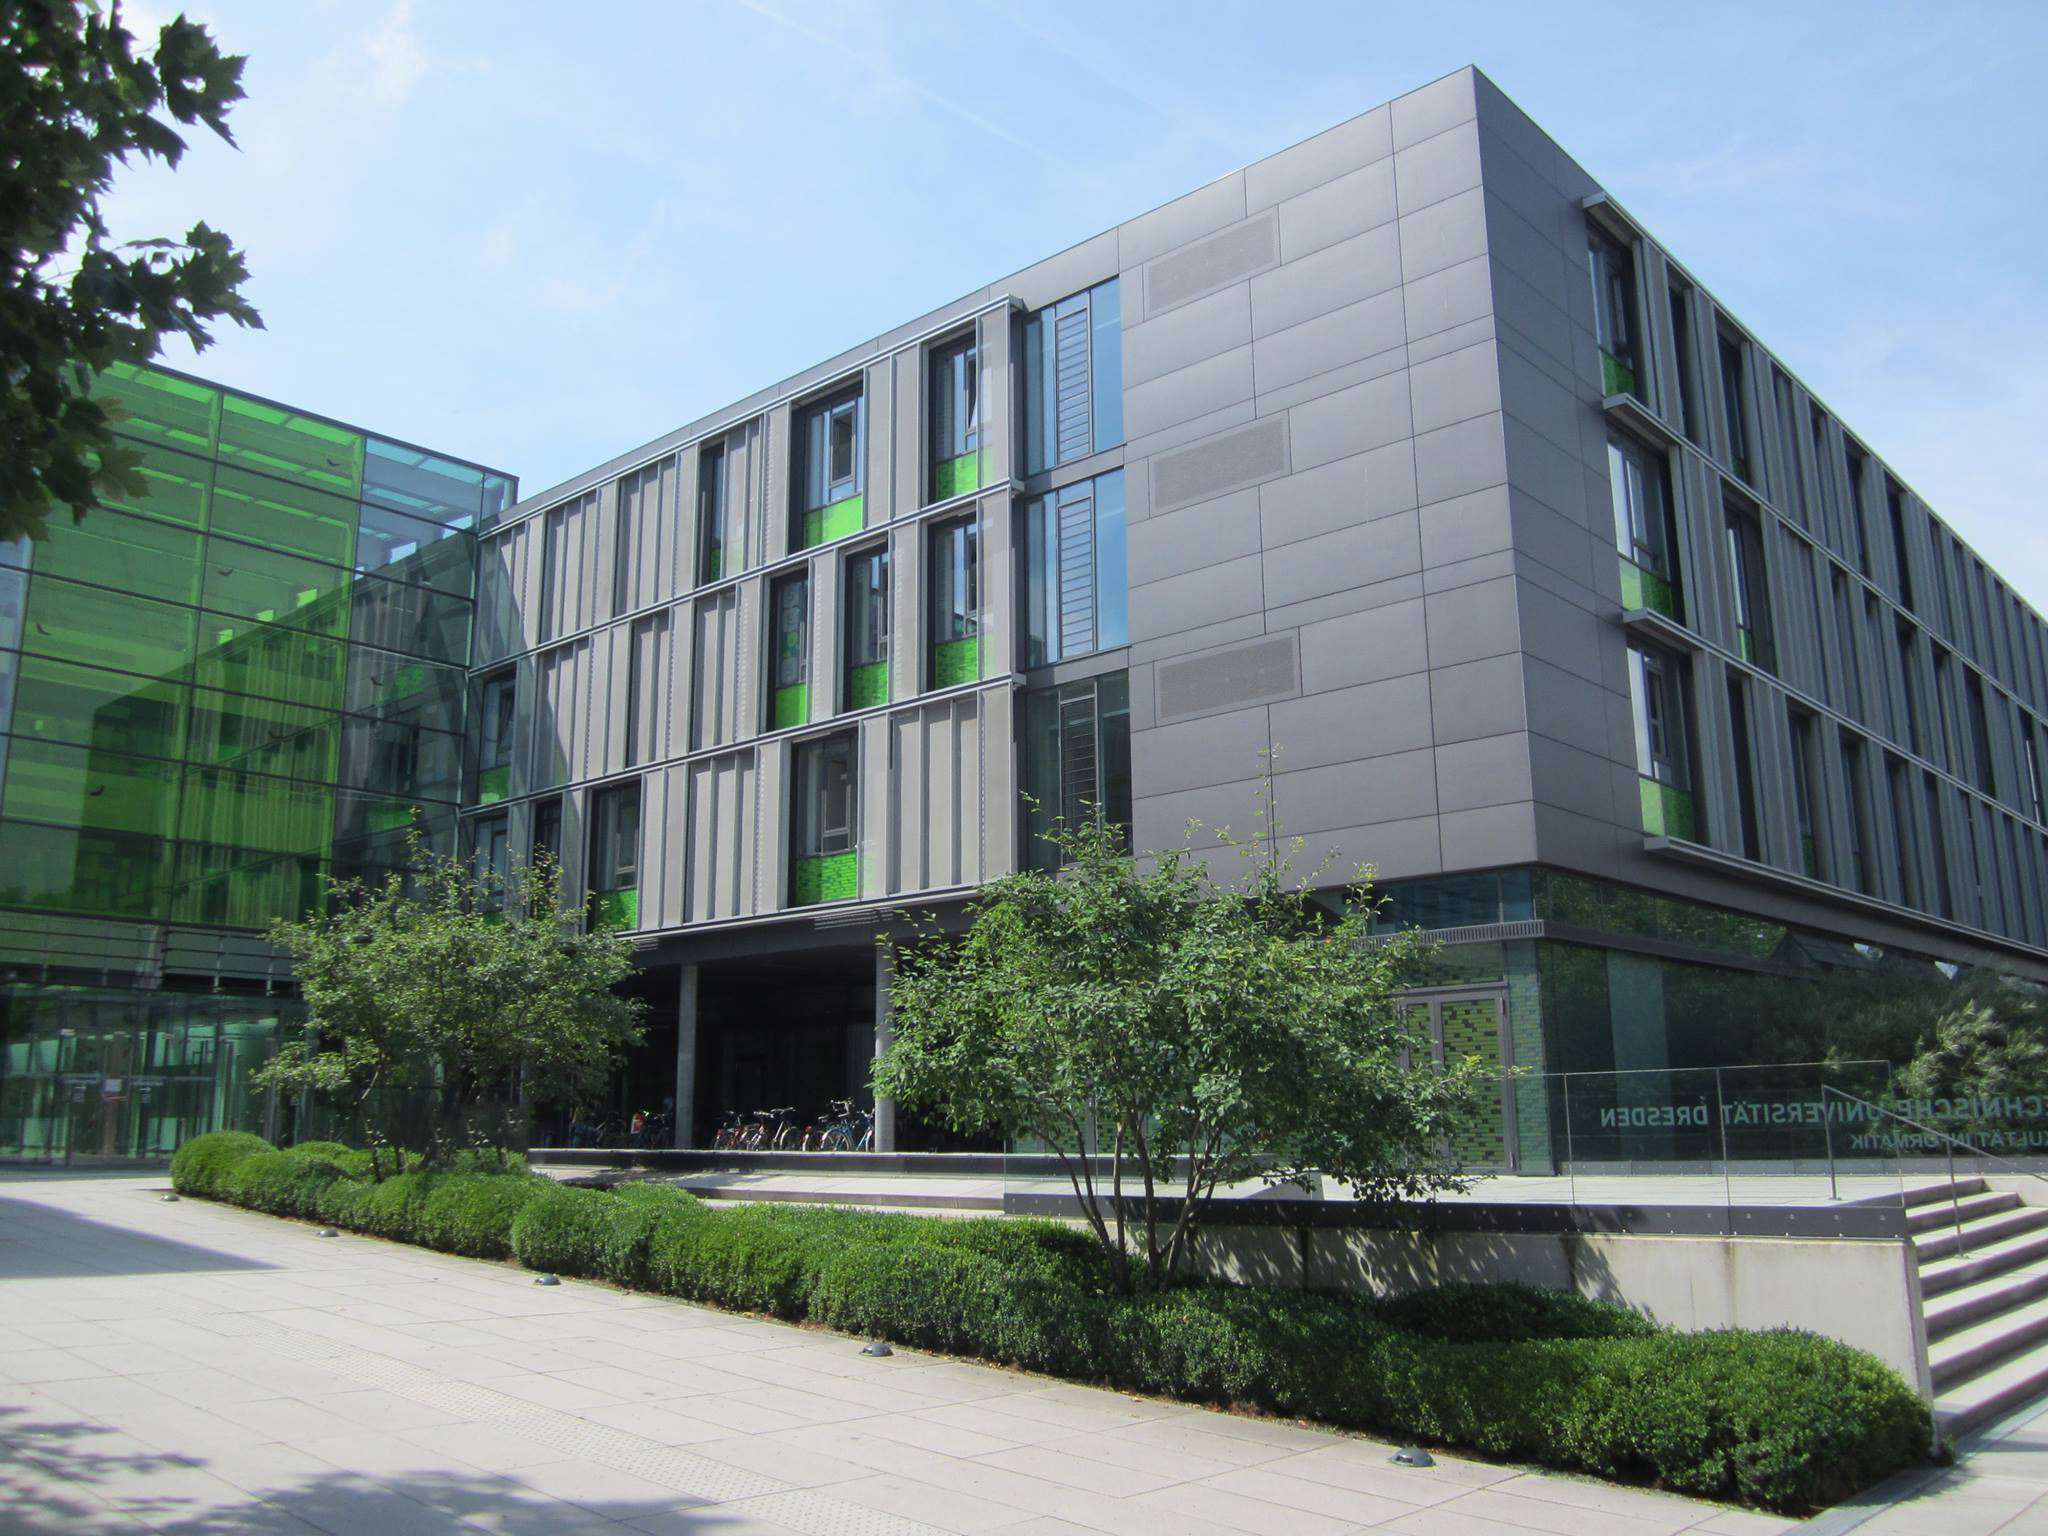
\includegraphics[width=\linewidth]{img/fakultaet.jpg}
\caption*{{\small Andreas-Pfitzmann-Bau (Fakultät Informatik) - Foto: Philipp Heisig}}
\end{figure}
%Bildlink: http://commons.wikimedia.org/wiki/File:TU-Dresden-Informatik.jpg
